The non-relativistic, Coulomb-interaction Hamiltonian for \h\ is given by 
\begin{equation}
\label{eq:H}
H = \frac{p_1^2}{2m_e} + \frac{p_2^2}{2m_e} - \frac{1}{4\pi\epsilon_0}\frac{e^2}{r_1} -  \frac{1}{4\pi\epsilon_0}\frac{e^2}{r_2} +  \frac{1}{4\pi\epsilon_0}\frac{e^2}{r_{12}}
\eeq
where $m_e$ is the mass of the electron, $p$ is the classical kinetic energy of the electron specified by the subscript, $e$ is the charge of the electron, $\epsilon_0$ is the vacuum permittivity, $r_1$ is the distance from the first electron to the nucleus, $r_2$ is the corresponding value for the second electron, and $r_{12}$ is the distance between the two electrons.  In this Hamiltonian the nucleus is assumed to be fixed.  This Hamiltonian possesses a term for each electron's kinetic energy, each electron's potential energy from its interaction with the nucleus (a single proton), and (specifically the last term in equation~\ref{eq:H}) a term for the repulsive Coulomb interaction between the two electrons.

Many approaches have been taken to calculate wavefunctions for \h.
Many-paramter Hylleraas functions are among the most commonly used.  I will focus on a simple two-parameter trial wavefunction used by \cite{chandra1944} because of the interpretations to which the simple wavefunction lends itself.  The wavefunction is
\beq
\label{eq:chandra}
\psi = \exp(-\alpha r_1 - \beta r_2) + \exp(-\alpha r_2 - \beta r_1).
\eeq
Chandrasekhar showed that the minimum energy of this wavefunction
($E_1=-0.51330$ at $\alpha = 1.03925$ and $\beta = 0.28309$) is
sufficient to provide binding for \h.  The wavefunction gives the
electrons a radial hierarchy, with one electron in close to the
nucleus and the other far away from the nucleus (which gives it its
correspondingly smaller binding energy). Chandrasekhar then, in the
same work, builds on the trial wavefunction in equation~\ref{eq:chandra} by
adding a term that accounts for the fact that one electron is
signficantly screened from the nucleus while the other electron is
practically unscreened, giving a trial wavefunction of the form
\beq
\label{eq:chandra2}
\psi = \left( e^{(-\alpha r_1 - \beta r_2)} + e^{(-\alpha r_2 - \beta r_1)} \right)
\times (1 + c r_{12}).
\eeq
% Additionally, the innermost electron
The energy is minimized with the values $a=1.07478,~b=0.47758,$ and
$c=0.31214$, giving an energy of $E_2=-0.52592$.  Chandrasekhar then
remarks that the addition of this term reduces the screening of the
outer electron (as can be seen by the fact that $E_2 < E_1$, showing
that the outermost electron is more bound in
equation~\ref{eq:chandra2} than in equation~\ref{eq:chandra}).  He
attributes this to the strong polarizability of the hydrogen atom (it
being just a single positive and a single negative charge, thus always
possesing a strong dipole component in the electric field).  A
classical picture of the \h\ ion is shown in
figure~\ref{fig:classical}. The radial hierarchy is seen, with a clear
inner and a clear outer electron.  This cartoon also provides a visual explanation of how the polarization of the H atom's electric field allows a second electron to bind: by positioning themselves opposite the nucleus from each other each electron is able to maximize its own Coulomb attraction to the nucleus in the presence of the other electron.
\begin{figure}
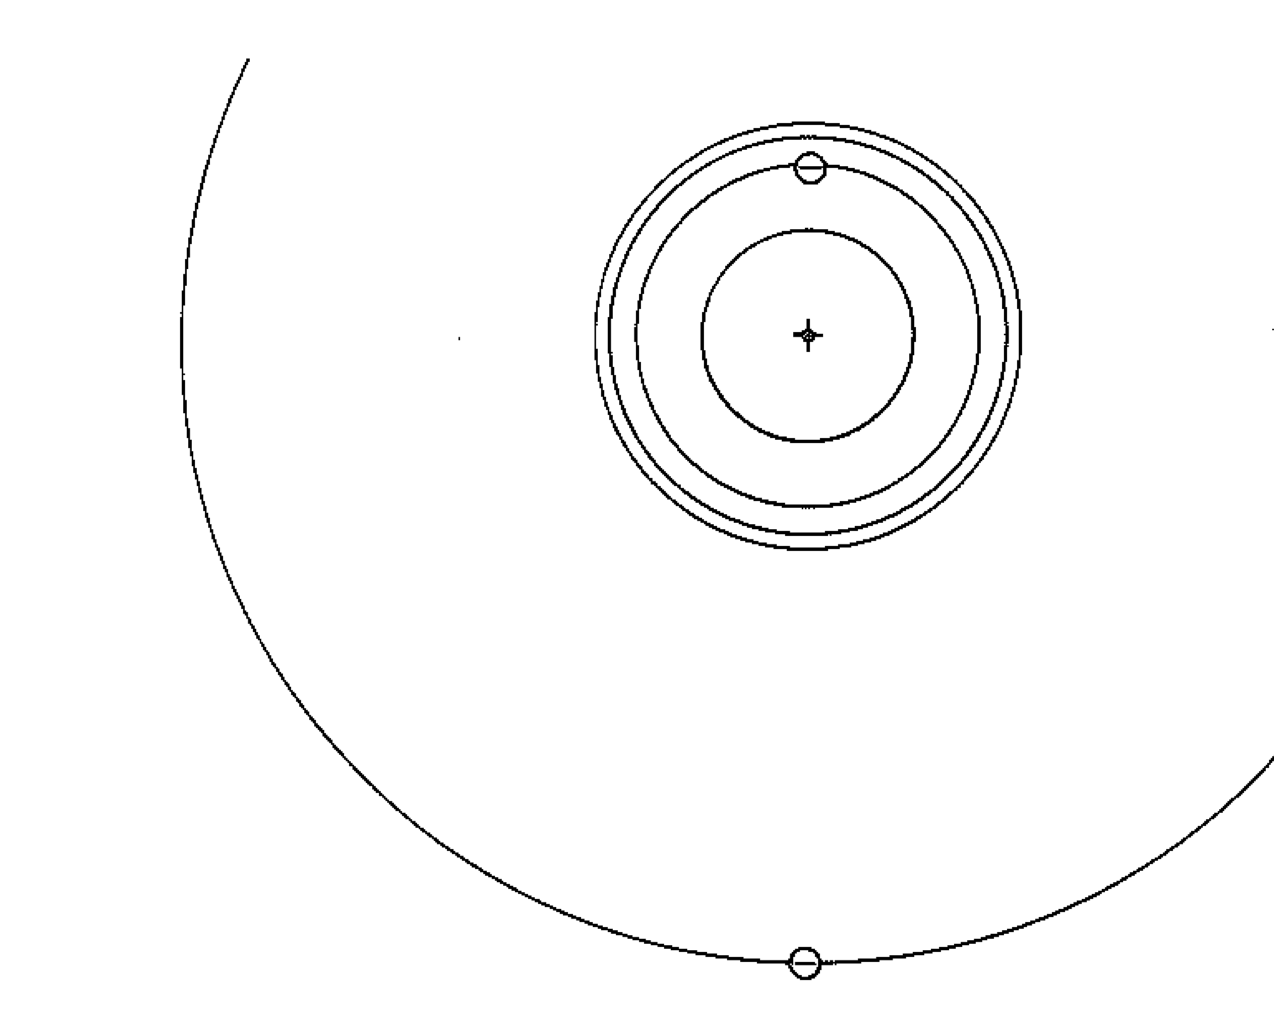
\includegraphics[width=\linewidth]{figs/classicalbohr.png}
\caption{\label{fig:classical}From \cite{collins1989}. A classical Bohr hydrogen atom with an additional electron bound to form an \h\ ion.}
\end{figure}

It has been rigorously shown that \h\ has no bound excited states,
i.e., the only bound state is the ground state (\citealt{hill1977}).
As such, \h\ does not have a line spectrum; there are no electronic transitions between bound states that absorb and emit photons of specific wavelengths.  Its main contribution to the opacity of the solar atmosphere is through continuum absorption of photons with energy greater than the binding energy of its least bound electron.  

The effect screening due to free electrons has on the binding energy of the \h\ ion has been looked at.  The partially ionized nature of the solar atmosphere makes this a relevant study.  \cite{phelpsbajaj1983} use a variational approach to show that the effect screening due to free electrons has on the binding energy of the \h\ ion is within a factor of 2 (as they quantify it) of the effect of screening on the binding energy of a single-electron H atom, despite the electron of the neutral H being $\sim 18$ times more bound than the least bound electron of \h.  To be specific, \cite{phelpsbajaj1983} 
%define a screening parameter $\delta$, where
%\beq
%\delta^2 = \sum_i \frac{4\pi n e^2}{k_B T}\left[ \frac{F_{-1/2}(\nu_i)}{F_{1/2}(\nu_i)}
%\eeq
assume a Dingle-Mansfield screening, which modifies equation~\ref{eq:H} to
\beq
H = \frac{p_1^2 + p_2^2}{2m_e} - \frac{1}{4\pi\epsilon_0}\frac{e^2}{r_1}e^{-\delta r_1} -  \frac{1}{4\pi\epsilon_0}\frac{e^2}{r_2}e^{-\delta r_2} + \\
 \frac{1}{4\pi\epsilon_0}\frac{e^2}{r_{12}} e^{-\delta r_{12}}
\eeq
where $\delta$ is a screening parameter defined in the text.  For my
purpose of comparison the exact definition of the screening parameter
is not necessary to include.  Their results are shown in
figure~\ref{fig:screening}.  They calculate that for  \h\ the binding
energy goes to zero for $a_0 \delta = 0.87$  (where $a_0$ is the Bohr
radius) while it is shown elsewhere that for H binding energy goes to
zero for $a_0 \delta = 1.2$ (\citealt{rogersetal1970}).  The two
values of $a_0 \delta$ are not very different which, as mentioned
previous, seems surprising due to the factor $~18$ discrepancy between
the binding energies of H and \h.  \cite{phelpsbajaj1983} attribute
this to the assumption that the interactions between the proton and
the electrons and the interaction between the electrons themselves are
modified in the presence of free electrons and so the ground state
energy is itself modified as a function of $\delta$; the binding
energy is modified by both the presence of free electrons and by the change in the ground state energy in the presence of free electrons.  The interplay of these two effects is what allows a perhaps intially surprisingly large value of $a_0 \delta$ for the binding energy to go to zero in \h.
\begin{figure}
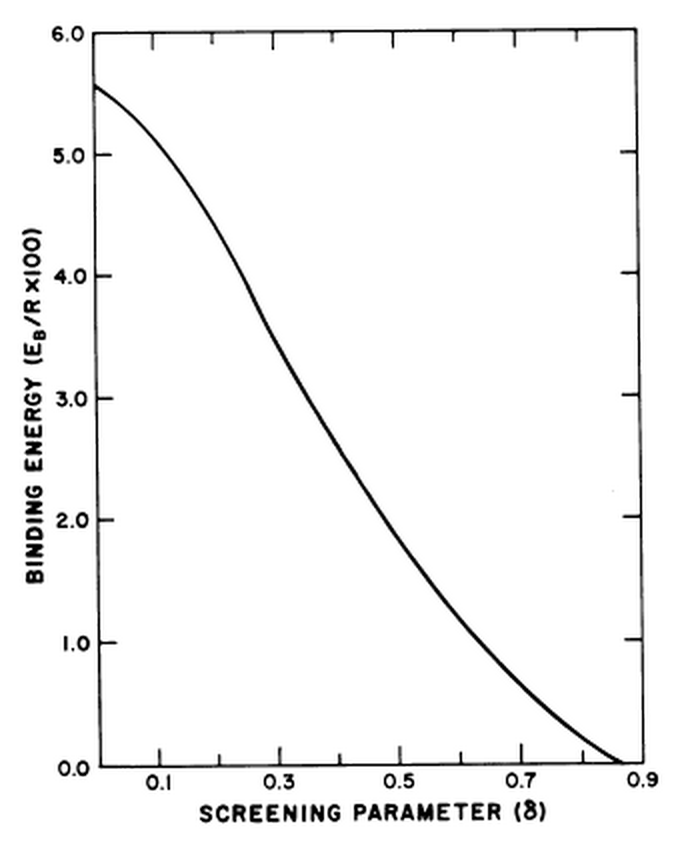
\includegraphics[width=76mm]{figs/screeningparameter.png}%normal width
                                %is 80mm
\caption{\label{fig:screening}From \cite{phelpsbajaj1983}. Binding energy of the least bound
electron in the \h\ ion as a function of screening parameter
$\delta$.  Binding energy is given in units of the Rydberg energy and
multiplied by 100.}
\end{figure}

To show the impact this screening has on \h\ opacity in the sun I will
reference figure~\ref{fig:screeninge}, taken from \cite{phelpsbajaj1983}.
The sun's photospheric temperature lies between the two temperature
curves of $4000K$ and $8000K$.  Simple order of magnitude arguments
will allow us to see that $\delta$ is small for the solar photosphere
without actually having to know the value for electron number
density.  The density of the photosphere is $\sim 1$ g/cm$^{-3}$, so
 there are Avogadro's number of electrons per cm$^{-3}$ in the
 photosphere, providing an upper limit of $\delta\sim 1$ based on
 figure~\ref{fig:screeninge}.  However, most electrons are still bound to
 their atoms in the photosphere.  \cite{boehm1989} calculates that
 the ionization fraction of H in the solar photosphere is $10^-4$.  H
 is the majority consituent of the solar photosphere; the next major
 constituent, He, has too large an ionization potential to be
 significantly ionized at these temperatures.  The metals of the
 photosphere have varying abundances and ionization states so it is
 less straightforward to calculate an ionization fraction for the
 metals, but since they only make up $\sim$1\%\ of the solar
 photosphere as long as their ionization fraction is less than
 $10^{-3}$ the metallic contribution will be comparable to that of H.
 This seems to be reasonable as an upper limit to the ionization
 fraction of metals, because, although some metals have lower
 ionization potentials than H, others have larger ionization
 potentials.  Additionally, ionization potential increases fairly
 sharply as a function of degree of ionization of an ion, so there is
 a low probability that metals will contribute more than one electron
 per atom/ion, for those species that do actually ionize.  With these
 arguments I set an upper limit on the free electron number density at
 $\sim 10^{19}$, which is $\sim 10^{-4} \times$ Avogadro's number.
 This gives a $\delta$ slightly larger than $10^{-2}$, which,
 referencing figure~\ref{fig:screening} shows the binding energy
 staying near its normal value of $0.754$ eV.  Thus screening from
 free electrons has a negligible but potentially measurable effect in
 the solar photosphere.

\begin{figure}
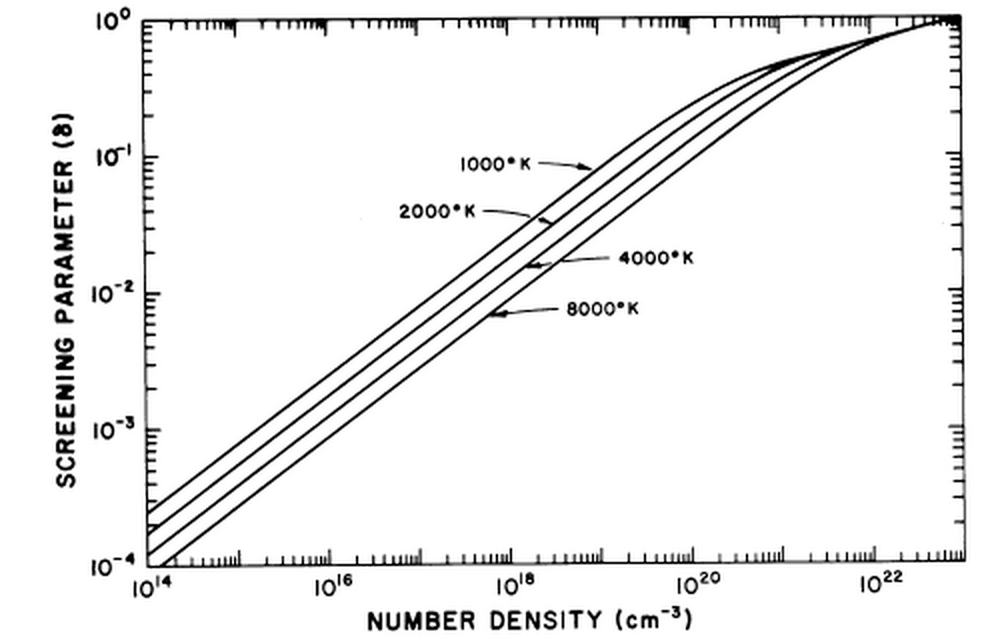
\includegraphics[width=\linewidth]{figs/screeningeffects.png}
\caption{\label{fig:screeninge}From \cite{phelpsbajaj1983}, shows the
screening parameter $\delta$ as a function of electron number density
for various temperatures.}
\end{figure}
